\section{Exploratory Data Analysis}

\subsection{Compiled Dataset Summary Statistics}

Each data set has a number of unique qualities and there is quite a bit of data to cover in order to have a thorough discussion of each nuance. Regardless there are still quite a few trends to consider before engaging in the model making. Note that unless otherwise specified, data here is from 2013, which is what we will use to create the slum mapping models as the training slums data set is from 2013 as well.


% latex table generated in R 4.0.3 by xtable 1.8-4 package
% Thu Mar 16 02:08:41 2023
\begin{table}[ht]
\centering
\caption{2013 Kenya Cleaned Data Summary Statistics}
\begin{tabular}{rlrrrrrrr}
  \hline \hline
 & habitation & total\_count & avg\_light & avg\_pop & sd\_light & sd\_pop\\ 
  \hline
1 & Not a Slum & 28986 & 0.67 & 189.60 & 2.50 & 301.45\\ 
  2 & Slum & 22381 & 2.39 & 137.63 & 8.03 & 430.09\\ 
  3 & Uninhabited & 1650 & 8.89 & 0.00 & 16.68\\ 
   \hline 
\end{tabular}
\end{table}

Table 2 indicates that our data set is slightly imbalanced. The ratio of slum to no slum observations in the training data is approximately 1:1.295 which is relatively much better than proportions if we were to process data from the entire country which would imbalance the data set to a ratio of about 1:16. Next, to discern the mixed effects of lights and population density, I engineer two new categorical variables by discretizing the range of both of these values into five quantiles; each of which is represented by a bin number, where the lower the bin number, the lower the quantile value. 

\begin{figure}
    \centering
    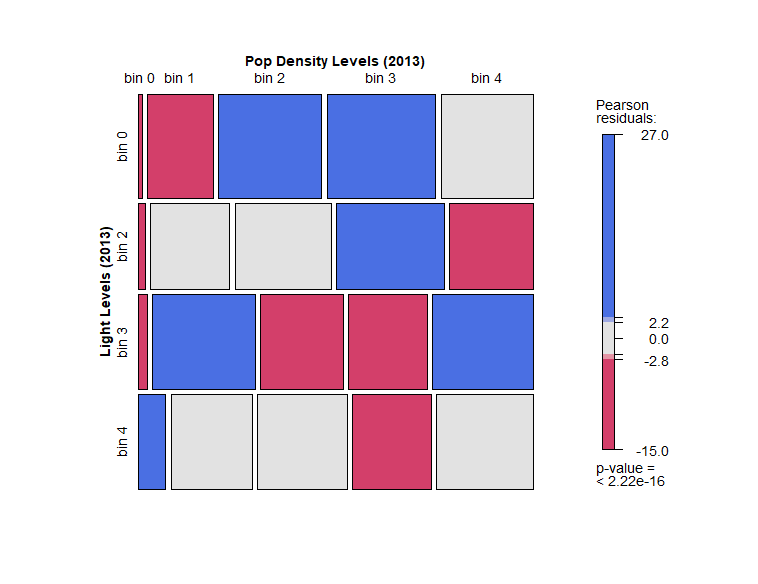
\includegraphics[scale = 0.36]{Graphics/Total Mosaic.png}
    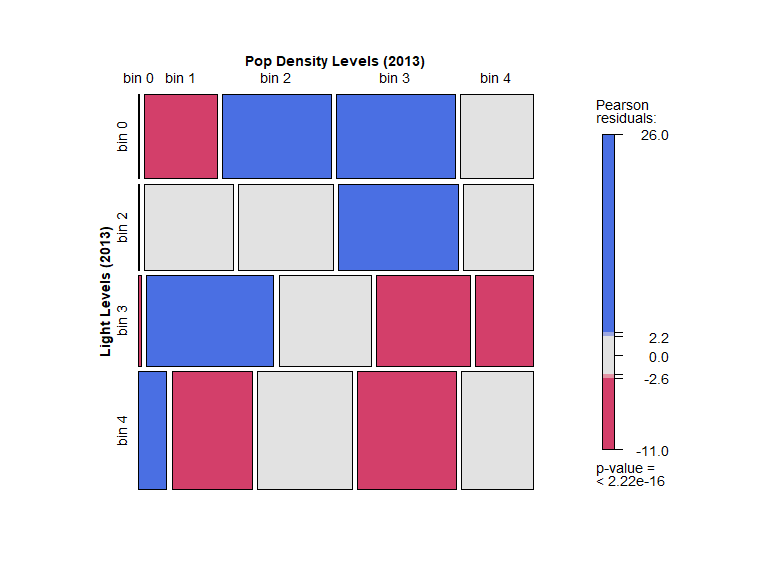
\includegraphics[scale = 0.36]{Graphics/Slum Mosaic.png}
    \caption{Distribution of lights and pop density values among slums is statistically biased}
    \label{fig:mosaic1}
\end{figure}

Before we delve into any of the model building, Figure 7 is a quick check for homogeneity of these categorical variables amongst both positive slum observations and the entire dataset. We can see some promising initial evidence that the distribution of slums does have a statistical bias towards low light levels and high population density, although there is also a few clusters at high light levels and low population density. At a qualitative level, the marginal distributions of the continuous population density and light values conditioned on a location being a slum or not seem to be about similar. But the sheer magnitude of the sample size reveals a different story when looking at statistical tests and show that there are indeed statistically significant differences in the means of the distribution and between the distribution as a whole at a 95\% confidence level.

\begin{table}[ht]
\centering
\caption{Distribution Tests}
\begin{tabular}{rlrrr}
  \hline \hline
 & Test & p-value & df & t-score \\ 
  \hline
1 & Two-sample Kolmogorov  & $<2.2e-16$ &  &   \\
 & Smirnov test & & &  \\
 \hline
  2 & Welch Two & $< 2.2e-16$ & 25752 & 30.849 \\
   & Sample T-test & & & \\
   \hline
\end{tabular}
\end{table}


\begin{figure}
    \centering
    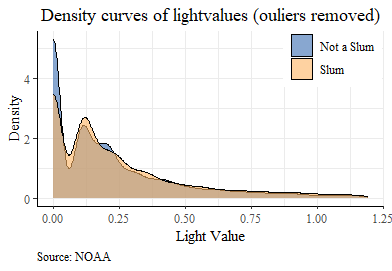
\includegraphics[scale = 0.7]{Graphics/Light Value density curve.png}
    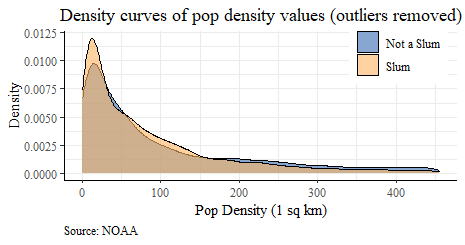
\includegraphics[scale = 0.75]{Graphics/Pop Density density curve.png}
    \caption{Distribution of lights and population density is heavily skewed towards smaller values}
    \label{fig:densitycurves}
\end{figure}

In the context of modeling, however, I discretize the continuous domain of light and population density values to capture the hypothesized non-linear effects of the interaction between population density and nighttime lights. For the basic model I break the light values into five quantiles and assign each observation's light value and population density value into a "bin" corresponding to their quantile. Figure 9 shows the distribution when we discretize the two features into ten bins: although population density seems to be approximately normally distributed with a high variance, the lights bins do not seem to be as well behaved as most light values tend to be very low and the bottom three quantiles are all the same.

\begin{figure}
    \centering
    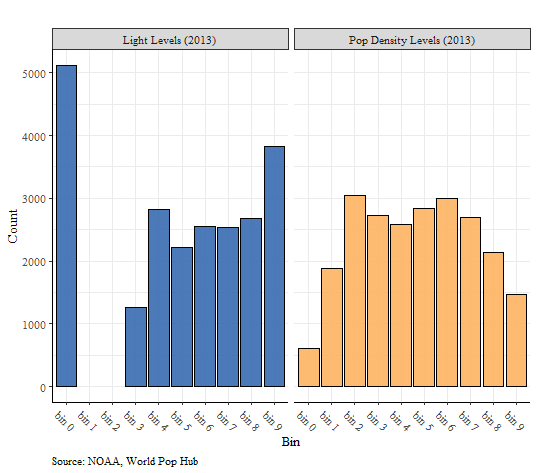
\includegraphics[scale = 0.7]{Graphics/10BinsBar.png}
    \caption{Caption}
    \label{fig:2013discretizeddistr}
\end{figure}

The benefit of increasing the number of bins is that we can capture a bit more non-linearity the models than with lower bins, but increasing the number of bins also has an added effect of potentially over-fitting and reducing the interpretability of the model: it no longer becomes a question of "low" and "high" light values but more so model effects contingent on individual bins and little insight into trends in the behavior of the data. It is important to note that the range of values, especially on the highest bin, may vary a lot due to outliers but cropping outliers can often times remove very key pieces of information since outliers in the context of this data often refers to city centers or very densely populated areas of a city which we have hypothesized may be home to slums.

\begin{figure}
    \centering
    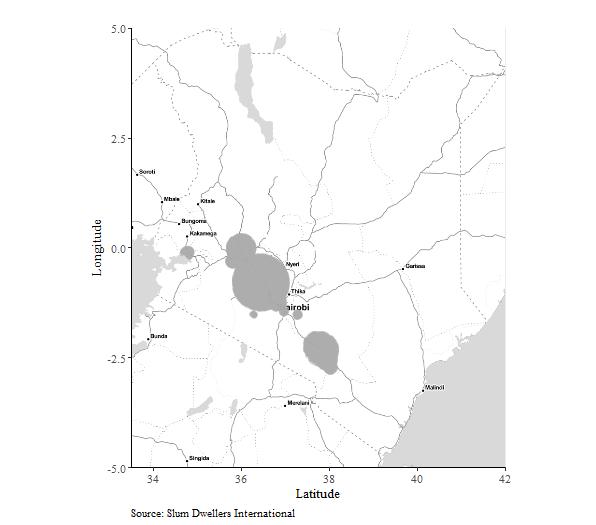
\includegraphics[scale = 0.6]{Graphics/Approximated Spatial Distribution of Slums in Kenya.png}
    \caption{Approximated Spatial Distribution of Slums in Kenya}
    \label{fig:slumMap}
\end{figure}

Finally, the data this paper works with is primarily spatial in nature: each observation is a latitude, longitude geo-coordinate pair. From an initial glance, we can clearly see assumptions about the shape of slums at play. Future iterations of the paper will embellish upon the slums data set and define more precise slum boundaries to better capture potential light and population density effects.


